\RequirePackage[l2tabu, orthodox]{nag}
\documentclass[12pt]{article}

\usepackage{amssymb,amsmath,verbatim,graphicx,microtype,upquote,units,booktabs,akkwidepage}

\newcommand{\chapterNumber}[1]{
    \setcounter{section}{#1}
    \addtocounter{section}{-1}
}

\title{Calculus III: Multivariable Calculus}
\author{Illya Starikov}
\date{\today}

\begin{document}
\maketitle
\tableofcontents\pagebreak

\chapterNumber{12}

\section{Vectors and Vector-Valued Functions}
\subsection{Vectors in the Plane}

\subsubsection{Vectors, Equal Vectors, Scalars, Zero Vector
}
\textbf{Vectors} are quantities that have both \textbf{length} (or \textbf{magnitude}) and \textbf{direction}. Two vectors are \textbf{equal} if they have the same magnitude and direction. Quantities having magnitude but no direction are called \textbf{scalars}. One exception is the \textbf{zero} vector, denoted \textbf{0}: It has length 0 and no direction.

\subsubsection{Scalar Multiples and Parallel Vectors}
Given a scalar $c$ and a vector \uvec, the scalar multiple $c$\vvec \ is a vector whose magnitude is $|c|$ multiplied by the magnitude of \vvec. If $c > 0$, then $c$\vvec has the same direction as \vvec. If $c < 0$, then $c$\vvec and \vvec point in opposite directions. Two vectors are \textbf{parallel} if they are scalar multiples of each other.

\subsubsection{Position Vectors and Vector Components}
A vector \vvec with its tail at the origin and head at the point $( v_1, v_2 )$ is called a \textbf{position vector} (or is said to be in \textbf{standard position}) and is written $\langle v_1, v_2 \rangle$. The real numbers $v_1$ and $v_2$ are the x- and y-\textbf{components} of \vvec, respectively. The position vectors $\uvec = \langle v_1, v_2 \rangle$ and $\vvec = \langle v_1, v_2 \rangle$ are equal if and only if $u_1 = v_1$ and $u_2 = v_2$.

\subsubsection{Magnitude of a Vector}
Given the points $P(x_1, y_1)$ and $Q(x_2, y_2)$, the \textbf{magnitude}, or \textbf{length}, of $\vec{PQ} = \langle x_2 - x_1, y_2 - y_1 \rangle$, denoted $|\vec{PQ}|$, is the distance between $P$ and $Q$:

\begin{equation}
    |\vec{PQ}| = \sqrt{ (x_2 - x_1)^2 + (y_2 - y_1)^2 }
\end{equation}

The magnitude of the position vector $\vvec = \langle v_1, v_2 \rangle$ is $|\vvec| = \sqrt{v_1^2 + v_2^2}$

\subsubsection{Vector Operations}
Suppose $\mathit{c}$ is a scalar, $\text{\uvec} = \langle u_1, u_2 \rangle$ and $\text{\vvec} = \langle v_1, v_2 \rangle$.

\begin{align}
    \uvec + \vvec &= \langle u_1 + v_1, u_2 + v_2 \rangle && \text{Vector addition} \\
    \uvec - \vvec &= \langle u_1 - v_1, u_2 - v_2 \rangle && \text{Vector subtraction} \\
    \mathit{c}\uvec &= \langle \mathit{c}u_1, \mathit{c} u_2 \rangle && \text{Scalar multiplication}
\end{align}

\subsubsection{Unit Vectors and Vectors of a Specified Length}
A \textbf{unit vector} is any vector with length 1. Given a nonzero vector $\vvec, \pm \frac{\vvec}{|\vvec|}$ are unit vectors parallel to $\vvec$. For a scalar $c > 0$, the vectors $\pm\frac{\mathit{c}\vvec}{|v|}$ are vectors of length $\mathit{c}$ parallel to $\vvec$.

\subsubsection{Properties of Vector Operations}
Suppose $\uvec, \vvec,$ and $\wvec$ are vectors and $a$ and $c$ are scalars. Then the following properties hold (for vectors in any number of dimensions).

\begin{align}
    \uvec + a = \vvec + \uvec && &\text{Commutative property of addition} \\
    (\uvec + \vvec) + \wvec = \uvec + (\vvec + \wvec) && &\text{Associative property of addition} \\
    \vvec + \mathbf{0} = \vvec && &\text{Additive identity} \\
    \vvec + (-\vvec) = 0 && & \text{Additive identity} \\
    c(\uvec + \vvec) = c\uvec + c\vvec && &\text{Distributive property 1} \\
    (a + c)\vvec = a\vvec + c\vvec && &\text{Distributive property 2} \\
    0\vvec = \mathbf{0} && &\text{Multiplication by zero scalar} \\
    c\mathbf{0} = \mathbf{0} && &\text{Multiplication by zero vector} \\
    1\vvec = \vvec && &\text{Multiplicative identity} \\
    a(c\vvec) = (ac)\vvec && &\text{Associative property of scalar multiplication}
\end{align}
\subsection{Vectors in Three Dimensions}
\subsubsection{Distance Formula in $xyz$-Space}
The distance between the points $P(x_1,\, y_1,\, z_1)$ and $Q(x_2,\, y_2,\, z_2)$ is

\begin{equation}
    \sqrt{(x_2 - x_1)^2 + (y_2 - y_1)^2 + (z_2 - z_1)^2}
\end{equation}

\subsubsection{Spheres and Balls}
A \textbf{sphere} centered at $(a,\, b,\, c)$ with radius $r$ is the set of points satisfying the
equation

\begin{equation}
    (x - a)^2 + (y - b)^2 + (z - c)^2 = r^2
\end{equation}

A ball centered at $(a,\, b,\, c)$ with radius $r$ is the set of points satisfying the inequality

\begin{equation}
    (x - a)^2 + (y - b)^2 + (z - c)^2 \leq r^2
\end{equation}

\subsubsection{Vector Operations in $\mathbb{R}$}
Let $c$ be a scalar, $\uvec = \langle u_1,\, u_2,\, u_3 \rangle$ and $\vvec = \langle v_1,\, v_2,\, v_3 \rangle$.

\begin{align}
    \uvec + \vvec = \langle u_1 + v_1,\, u_2 + v_2,\, u_3 + v_3 \rangle && &\text{Vector addition} \\
    \uvec - \vvec = \langle u_1 - v_1,\, u_2 - v_2,\, u_3 - v_3 \rangle && &\text{Vector subtraction} \\
    c\uvec = \langle c u_1,\, c u_2,\, c_3 \rangle
\end{align}

\subsubsection{Magnitude of a Vector}
The \textbf{magnitude} (or \textbf{length}) of the vector $\vec{PQ} = \langle x_2 - x_1,\, y_2 - y_1,\, z_2 - z_1 \rangle$ is the distance from $P(x_1,\, y_1,\, z_1)$ to $Q(x_2,\, y_2,\, z_2)$

\begin{equation}
    |\vec{PQ}| = \sqrt{(x_2 - x_1)^2 + (y_2 - y_1)^2 + (z_2 - z_1)^2}
\end{equation}

\subsection{Dot Product}
\subsubsection{Dot Product}
Given two nonzero vectors \uvec \ and \vvec \ in two or three dimensions, their \textbf{dot product} is

\begin{equation}
    \uvec \cdot \vvec = |\uvec||\vvec| \cos \theta
\end{equation}

where $\theta$ is the angle between \uvec and \vvec with $0 \leq \theta \leq \pi$. If $\uvec = \mathbf{0}$ or $\vvec = \mathbf{0}$, then $\uvec \cdot \vvec = 0$, and $\theta$ is undefined.

\subsubsection{Orthogonal Vectors}
Two vectors \uvec and \vvec are \textbf{orthogonal} if and only if $\uvec \cdot \vvec = 0$. The zero vector is orthogonal to all vectors. In two or three dimensions, two nonzero orthogonal vectors are perpendicular to each other.

\subsubsection{Dot Product}
Given two vectors $\uvec = \langle u_1,\, u_2,\, u_3 \rangle$ and $\vvec = \langle v_1,\, v_2,\, v_3 \rangle$,

\begin{equation}
    \uvec \cdot \vvec = u_1v_1 + u_2v_2 + u_3v_3
\end{equation}

\subsubsection{Properties of the Dot Product}
Suppose \uvec, \vvec, and \wvec are vectors and let $c$ be a scalar.

\begin{align}
    \uvec \cdot \vvec = \vvec \cdot \uvec && &\text{Commutative property} \\
    c(\uvec \cdot \vvec) = (c\uvec) \cdot \vvec = \uvec \cdot (c \vvec) && &\text{Associative property} \\
    \uvec \cdot (\vvec + \wvec) = \uvec \cdot \vvec + \uvec \cdot \wvec
\end{align}

\subsubsection{(Orthogonal) Projection of u onto v}
The \textbf{orthogonal projection of \uvec onto \vvec}, denoted $\text{proj}_{\vvec}\uvec$, where $\vvec \neq \mathbf{0}$, is

\begin{equation}
    \text{proj}_{\vvec}\uvec = |\uvec| \cos \theta \Bigg( \frac{\vvec}{|\vvec|} \Bigg)
\end{equation}

The orthogonal projection may also be computed with the formulas

\begin{equation}
    \text{proj}_{\vvec}\uvec = \text{scal}_{\vvec}\uvec \Bigg( \frac{\vvec}{|\vvec|} \Bigg) = \Bigg( \frac{\uvec \cdot \vvec}{\vvec \cdot \vvec} \Bigg)\vvec
\end{equation}

where the \textbf{scalar component of u in the direction of \vvec} is

\begin{equation}
    \text{scal}_{\vvec}\uvec = |\uvec| \cos \theta = \frac{\uvec \cdot \vvec}{|\vvec|}
\end{equation}

\subsubsection{Work}
Let a constant force \textbf{F} be applied to an object, producing a displacement \textbf{d}. If the angle between \textbf{F} and \textbf{d} is $\theta$, then the \textbf{work} done by the force is

\begin{equation}
    W = \mathbf{|F||d|} \cos \theta = \mathbf{F \cdot d}
\end{equation}

\subsection{Cross Product}
Given two nonzero vectors \uvec \ and \vvec \ in $\mathbb{R}^3$, the \textbf{cross product} $\uvec \times \vvec$ is a vector with magnitude

\begin{align}
    |\uvec \times \vvec| = |\uvec||\vvec| \sin \theta
\end{align}

where $0 \leq \theta \leq \pi$ is the angle between \uvec and \vvec. The direction of $\uvec \times \vvec$ is given by the \textbf{right-hand rule}: When you put the vectors tail to tail and let the fingers of your right hand curl from \uvec to \vvec the direction of $\uvec \times \vvec$ is the direction of your thumb, orthogonal to both \uvec and \vvec. When $\uvec \times \vvec = 0$, the direction of $\uvec \times \vvec$ undefined.

\subsubsection{Geometry of the Cross Product}
Let \uvec and \vvec be two nonzero vectors in $\mathbb{R}^3$.

\begin{enumerate}
    \item The vectors \uvec and \vvec are parallel ($\theta = 0$ or $\theta = \pi$) if and only if $\uvec \times \vvec = 0$.
    \item If \uvec and \vvec are two sides of a parallelogram, then the area of the parallelogram is

    \begin{align}
        |\uvec \times \vvec| = |\uvec||\vvec| \sin \theta
    \end{align}
\end{enumerate}

\subsubsection{Properties of the Cross Product}
Let \uvec, \vvec, and \wvec be nonzero vectors in $\mathbb{R}^3$, and let $a$ and $b$ be scalars.

\begin{align}
    \uvec \times \vvec = -(\vvec \times \uvec) && &\text{Anticommutative property} \\
    (a \uvec) \times (b \vvec) = ab(\uvec \times \vvec) && &\text{Associative property} \\
    \uvec \times (\vvec + \wvec) = (\uvec \times \vvec) + (\uvec \times \wvec) && &\text{Distributive property} \\
    (\uvec + \vvec) \times \wvec = (\uvec \times \wvec) + (\vvec \times \wvec) && &\text{Distributive property}
\end{align}

\subsubsection{Cross Products of Coordinate Unit Vectors}
\begin{center}
    \tdplotsetmaincoords{60}{125}
    \begin{tikzpicture}
            [tdplot_main_coords,
                cube/.style={very thick,black},
                grid/.style={very thin,gray},
                axis/.style={->,blue,thick}]

        %draw a grid in the x-y plane
        \foreach \x in {-1.5,0,...,3.5}
            \foreach \y in {-1.5,0,...,3.5}
            {
                \draw[grid] (\x,-1.5) -- (\x,3.5);
                \draw[grid] (-1.5,\y) -- (3.5,\y);
            }


        %draw the axes
        \draw[axis] (0,0,0) -- (5,0,0) node[anchor=west]{$x = \ihat$};
        \draw[axis] (0,0,0) -- (0,5,0) node[anchor=west]{$y = \jhat$};
        \draw[axis] (0,0,0) -- (0,0,5) node[anchor=west]{$z = \khat$};
        \end{tikzpicture}
\end{center}

\begin{align}
    \ihat \times \jhat &= -(\jhat \times \ihat) = \khat \\
    \jhat \times \khat &= -(\khat \times \jhat) = \ihat \\
    \khat \times \ihat &= -(\ihat \times \khat) = \jhat \\
    \ihat \times \ihat &= \jhat \times \jhat = \khat \times \khat = 0
\end{align}

\subsubsection{Evaluating the Cross Product}
Let $\uvec = u_1\ihat + u_2\jhat + u_3\khat$ and $\vvec = v_1\ihat + v_2\jhat + v_3\khat$. Then

\begin{equation}
    \uvec \times \vvec
    = \begin{vmatrix} \ihat & \jhat & \khat \\ u_1 & u_2 & u_3 \\ v_1 & v_2 & v_3 \end{vmatrix}
    = \begin{vmatrix} u_2 & u_3 \\ v_2 & v_3 \end{vmatrix}\ihat
    - \begin{vmatrix} u_1 & u_3 \\ v_1 & v_3 \end{vmatrix}\jhat
    + \begin{vmatrix} u_1 & u_2 \\ v_1 & v_2 \end{vmatrix}\khat
\end{equation}
\subsection{Lines and Curves in Space}
\subsubsection{Equation of a Line}
An equation of the line passing through the point $P_0(x_0,\, y_0,\, z_0)$ in the direction of the vector $\vvec = \langle a,\, b,\, c \rangle$ is $\mathbf{r} = r_0 + t\vvec$, or

\begin{equation}
    \langle x,\, y,\, z \rangle = \langle x_0,\, y_0,\, z_0 \rangle + t \langle a,\, b,\, c \rangle, \quad \text{for} \quad -\infty < t < \infty
\end{equation}

Equivalently, the parametric equations of the line are

\begin{equation}
    x = x_0 + at, \quad
    y = y_0 + bt, \quad
    z = z_0 + ct, \quad
    \text{for} \quad -\infty < t < \infty
\end{equation}

\subsubsection{Limit of a Vector-Valued Function}
A vector-valued function \textbf{r} approaches the limit \textbf{L} as $t$ approaches $a$, written $\limit{t \to a} \mathbf{r}(t) = \mathbf{L}$, provided $\limit{t \to a}|\mathbf{r}(t) - \mathbf{L}| = 0$

\subsection{Calculus of Vector-Valued Functions}
\subsubsection{Derivative and Tangent Vector}
Let $\mathbf{r}(t) = f(t)\ihat + g(t)\jhat + h(t)\khat$, where $f$, $g$, and $h$ are differentiable functions on $(a\, b)$. Then \textbf{r} has a \textbf{derivative} (or is \textbf{differentiable}) on $(a\, b)$ and

\begin{equation}
    \mathbf{r}'(t) = f'(i)\ihat + g'(t)\jhat + h'(t)\khat
\end{equation}

Provided $\mathbf{r}'(t) \neq \mathbf{0}, \mathbf{r}'(t)$ is a \textbf{tangent vector} (or velocity vector) at the point corresponding to $\mathbf{r}$.

\subsubsection{Unit Tangent Vector}
Let $\mathbf{r} = f(t)\ihat + g(t)\jhat + h(t)\khat$ be a smooth parameterized curve, for $a \leq t \leq b$. The \textbf{unit tangent vector} for a particular value of $t$ is

\begin{equation}
    \mathbf{T}(t) = \frac{\mathbf{r}'(t)}{|\mathbf{r}'(t)|}
\end{equation}

\subsubsection{Derivative Rules}
Let \uvec and \vvec be differentiable vector-valued functions and let $f$ be a differentiable scalar-valued function, all at a point $t$. Let \textbf{c} be a constant vector. The following rules apply.

\begin{align}
    \frac{d}{dt} (\mathbf{c}) = \mathbf{0}   && &\text{Constant Rule} \\
    \frac{d}{dt} (\uvec(t) + \vvec(t)) = \uvec'(t) + \vvec'(t)   && &\text{Sum Rule} \\
    \frac{d}{dt} (f(t) \uvec(t)) = f'(t) \uvec(t) + f(t) \uvec'(t)   && &\text{Product Rule} \\
    \frac{d}{dt} (\uvec (f(t))) = \uvec'(f(t)) f'(t)   && &\text{Chain Rule} \\
    \frac{d}{dt} (\uvec(t) \cdot \vvec(t)) = \uvec'(t) \cdot \vvec(t) + \uvec(t) \cdot \vvec'(t)   && &\text{Dot Product Rule} \\
    \frac{d}{dt} (\uvec(t) \times \vvec(t)) = \uvec'(t) \times \vvec(t) + \uvec(t) \times \vvec'(t)   && &\text{Cross Product Rule}
\end{align}

\subsubsection{Indefinite Integral of a Vector-Valued Function}
Let $\mathbf{r} = f\ihat + g\jhat + h\khat$ be a vector function and let $\mathbf{R} = F\ihat + G\jhat + H\khat$, where $F$, $G$, and $H$ are antiderivatives of $f$, $g$, and $h$, respectively. The \textbf{indefinite integral} of \textbf{r} is

\begin{equation}
    \int \mathbf{r}(t) \, dt = \mathbf{R}(t) + \mathbf{C}
\end{equation}

where \textbf{C} is an arbitrary constant vector.

\subsubsection{Definite Integral of a Vector-Valued Function}
Let $\mathbf{r}(t) = f(t)\ihat + g(t)\jhat + h(t)\khat$, where $f$, $g$, and $h$ are integrable on the interval $[a,\, b]$.

\begin{equation}
    \int \mathbf{r}(t) \, dt =
    \Bigg[ \int _a ^b f(t) \, dt \Bigg] \ihat +
    \Bigg[ \int _a ^b g(t) \, dt \Bigg] \jhat +
    \Bigg[ \int _a ^b h(t) \, dt \Bigg] \khat
\end{equation}

\subsection{Motion In Space}
\subsubsection{Position, Velocity, Speed, Acceleration}
Let the position of an object moving in three-dimensional space be given by $\mathbf{r}(t) = \langle x(t), y(t), z(t) \rangle$, for $t \geq 0$. The \textbf{velocity} of the object is

\begin{equation}
    \vvec(t) = \mathbf{r}'(t) = \langle x'(t), y'(t), z'(t) \rangle
\end{equation}

The \textbf{speed} of the object is the scalar function

\begin{equation}
    |\vvec(t)| = \sqrt{x'(t)^2 + y'(t)^2 + z'(t)^2}
\end{equation}

The \textbf{acceleration} of the object is $\mathbf{a}(t) = \mathbf{v}'(t) = \mathbf{r}''(t)$.

\subsubsection{Motion with Constant $\vert \mathbf{r} \vert$}
Let \textbf{r} describe a path on which $\vert \mathbf{r} \vert$ is constant (motion on a circle or sphere centered at the origin). Then, $\mathbf{r \cdot v} = 0$, which means the position vector and the velocity vector are orthogonal at all times for which the functions are defined.

\subsubsection{Two-Dimensional Motion in a Gravitational Field}
Consider an object moving in a plane with horizontal $x$-axis and a vertical $y$-axis, subject only to the force of gravity. Given the initial velocity $\vvec(0) = \langle u_0,\, v_0 \rangle$ and the initial position $\mathbf{r}(0) = \langle x_0,\, y_0 \rangle$, the velocity of the object, for $t \geq 0$, is

\begin{equation}
    \mathbf{v}(t) = \langle x'(t),\, y'(t) \rangle = \langle u_0,\, -gt + v_0 \rangle
\end{equation}

and the position is

\begin{equation}
    \mathbf{r}(t) = \langle x(t),\, y(t) \rangle = \Bigg \langle u_0 \ t + x_0,\, -\frac{1}{2} gt^2 + v_0 t + y_0 \Bigg \rangle
\end{equation}

\subsubsection{Two-Dimensional Motion}
Assume an object traveling over horizontal ground, acted on only by the gravitational force, has an initial position $\langle x_0,\, y_0 \rangle = \langle 0,\, 0 \rangle$ and initial velocity $\langle u_0,\, v_0 \rangle = \langle |\vvec_0|\cos\alpha,\, |\vvec_0|\sin\alpha \rangle$. The trajectory, which is a segment or a parabola, has the following properties.

\begin{align}
    \text{time of flight} &= T = \frac{2|\vvec_0|\sin\alpha}{g} \\
    \text{range} &= \frac{|\vvec_0|\sin 2\alpha}{g} \\
    \text{maximum height} &= y \Bigg( \frac{T}{2} \Bigg) = \frac{(|\vvec_0| \sin \alpha)^2}{2g}
\end{align}

\subsection{Length of Curves}
Consider the parameterized curve $\mathbf{r}(t) = \langle f(t), g(t), h(t) \rangle$, where $f'$, $g'$, and $h'$ are continuous, and the curve is traversed once for $a \leq t \leq b$. The \textbf{arc length} of the curve between $(f(a), g(a), h(a))$ and $(f(b), g(b), h(b))$ is

\begin{equation}
    L = \int _a ^b \sqrt{f'(t)^2 + g'(t)^2 + h'(t)^2} \, dt = \int _a ^b |\mathbf{r'(t)}|\, dt
\end{equation}

\subsubsection{Arc Length of a Polar Curve}
Let $f$ have a continuous derivative on the interval $[\alpha, \beta]$. The \textbf{arc length} of the polar curve $r = f(\theta)$ on $[ \alpha,\, \beta ]$ is

\begin{equation}
    L = \int _\alpha ^\beta \sqrt{f(\theta)^2 + f'(\theta)^2} \, d\theta.
\end{equation}

\subsubsection{Arc Length as a Function of a Parameter}
Let \textbf{r}(t) describe a smooth curve, for $t \geq a$. The arc length is given by

\begin{equation}
    s(t) = \int _a ^t |\vvec(u)| \, du,
\end{equation}

where $|\vvec| = |\mathbf{r'}|$. Equivalently, $\frac{ds}{dt} = |\vvec{t}| > 0$. If $|\vvec(t)| = 1$, for all $t \geq a$, then the parameter $t$ corresponds to arc length.

\subsubsection{Arc Length as a Function of a Parameter}
Let \textbf{r}(t) describe a smooth curve, for $t \geq a$. The arc length is given by

\begin{equation}
    s(t) = \int _a ^t |\vvec(u) | \, du,
\end{equation}

where $|\vvec| = |\mathbf{r}'|$. Equivalently, $\frac{ds}{dt} = \vvec(t) > 0$. If $|\mathbf{v(t)}| = 1$, for all $t \geq a$, then the parameter $t$ corresponds to arc length.

\subsection{Curvature and Normal Vectors}
\subsubsection{Curvature}
Let \textbf{r} describe a smooth parameterized curve. If $s$ denotes arc length and $\mathbf{T} = \mathbf{\frac{r'}{|r'|}}$ is the unit tangent vector, the \textbf{curvature} is $\kappa(s) = |\frac{d\mathbf{T}}{ds}|$

\subsubsection{Curvature Formula}
Let $\mathbf{r}(t)$ describes a smooth parameterized curve, where $t$ is any parameter. If $\vvec = \mathbf{r}'$ is the velocity and \textbf{T} is the unit tangent vector, then the curvature is

\begin{equation}
    \kappa (t) = \frac{1}{|\mathbf{v}|}\Bigg|\frac{d \mathbf{T}}{dt}\Bigg| = \Bigg|\frac{\mathbf{T}'(t)}{\mathbf{r}'(t)}\Bigg|
\end{equation}

\subsubsection{Alternative Curvature Formula}
Let \textbf{r} be the position of an object moving on a smooth curve. The \textbf{curvature} at a point on the curve is

\begin{equation}
    \kappa = \frac{|\mathbf{v \times a}|}{|\mathbf{v}|^3},
\end{equation}

where $\mathbf{v} = \mathbf{r}'$ is the velocity and $\mathbf{a} = \mathbf{v}'$ is the acceleration.

\subsubsection{Principal Unit Normal Vector}
Let \textbf{r} describe a smooth parameterized curve. The \textbf{principal unit normal vector} at a point $P$ on the curve at which $\kappa \neq 0$ is

\begin{equation}
    \mathbf{N}(s)
    = \frac{ \nicefrac{d \mathbf{T}}{ds} }{| \nicefrac{d \mathbf{T}}{ds} |}
    = \frac{1}{\kappa} \frac{d \mathbf{T}}{ds}
\end{equation}

In practice, we use the equivalent formula

\begin{equation}
    \mathbf{N}(t) = \frac{ \nicefrac{d \mathbf{T}}{dt} }{| \nicefrac{d \mathbf{T}}{dt} |}
\end{equation}

evaluated at the value of $t$ corresponding to $P$.

\subsubsection{Properties of the Principal Unit Normal Vector}
Let \textbf{r} describe a smooth parameterized curve with unit tangent vector \textbf{T} and principal unit normal vector \textbf{N}.

\begin{enumerate}
    \item \textbf{T} and \textbf{N} are orthogonal at all points of the curve; that is, $\mathbf{T}(t) \cdot \mathbf{N}(t) = 0$, at all points where \textbf{N} is defined.
    \item The principal unit normal vector points to the inside of the curve---in the direction that the curve is turning.
\end{enumerate}

\subsubsection{Tangential and Normal Components of the Acceleration}
The acceleration vector of an object moving in space along a smooth curve has the following representation in terms of its \textbf{tangential component} $a_T$ (in the direction of \textbf{T}) and its normal component $a_N$ (in the direction of \textbf{N}):

\begin{equation}
    \mathbf{a} = a_N \mathbf{N} + a_T \mathbf{T},
\end{equation}

where $a_N = \kappa |\vvec|^2 = \frac{|\mathbf{v \times a}|}{|\vvec|}$ and $a_T = \frac{d^2 s}{dt^2}$.

\subsubsection{Unit Binormal Vector and Torsion}
Let $C$ be a smooth parameterized curve with unit tangent and principal unit normal vectors \textbf{T} and \textbf{N}, respectively. Then, at each point of the curve at which the curvature is nonzero, the \textbf{unit binormal vector} is

\begin{equation}
    \mathbf{B} = \mathbf{T \times N}
\end{equation}

and the \textbf{torsion} is

\begin{equation}
    \tau = - \frac{d \textbf{B}}{ds} \cdot \mathbf{N}
\end{equation}

\subsubsection{Formulas for Curves in Space}
\begin{enumerate}
    \item Position function: $\quad \mathbf{r}(t) = \langle x(t),\, y(t),\, z(t) \rangle$
    \item Velocity: $\quad \mathbf{v} = \mathbf{r}'$
    \item Acceleration: $\quad \mathbf{a} = \mathbf{v}'$
    \item Unit tangent vector: $\quad \mathbf{T} = \frac{\mathbf{v}}{|\mathbf{v}|}$
    \item Principal unit normal vector: $\quad \mathbf{N} = \frac{ \nicefrac{d \mathbf{T}}{dt} }{| \nicefrac{d \mathbf{T}}{dt} |}$ (provided $\nicefrac{d \mathbf{T}}{dt} \neq \mathbf{0}$)
    \item Curvature: $\quad \kappa = \frac{d \mathbf{T}}{ds} = \frac{1}{|\mathbf{v}|}|\frac{d \mathbf{T}}{dt}| = |\frac{\mathbf{T}'(t)}{\mathbf{r}'(t)}| = \frac{| \vvec \times \mathbf{a}|}{|\vvec|^3}$
    \item Components of acceleration: $\quad \mathbf{a} = a_N \mathbf{N} + a_T \mathbf{T}$, where $a_N = \kappa |\mathbf{v}|^2 = \frac{|\vvec \times \mathbf{a}|}{|\mathbf{v}|}$ and $a_T = \frac{d^2 s}{dt^2} = \frac{\mathbf{v \cdot a}}{|\mathbf{v}|}$
    \item Unit binormal vector: $\mathbf{B} = \mathbf{B \times N} = \frac{\mathbf{v \times a}}{|\mathbf{v \times a}|}$
    \item Torsion $\quad \tau = -\frac{d \mathbf{B}}{ds} \cdot \mathbf{N} = \frac{ \mathbf{(v \times a)} \cdot \mathbf{a}' }{|\mathbf{v \times a}|^2} = \frac{\mathbf{(r' \times r'') \cdot r'''}}{(\mathbf{r}' \times \mathbf{r}'')^2}$
\end{enumerate}


\section{Functions of Several Variables}
\subsection{Planes and Surfaces}
\subsubsection{Plane in $\mathbb{R}^3$}
Given a fixed point $P_0$ and a nonzero \textbf{normal vector n}, the set of points $P$ in $\mathbb{R}^3$ for which $\vec{P_0 P}$ is orthogonal to $\mathbf{n}$ is called a \textbf{plane}.

\subsubsection{General Equation of a Plane in $\mathbb{R}^3$}
The plane passing through the point $P_0 (x_0,\, y_0,\, z_0)$ with a nonzero normal vector $\mathbf{n} = \langle a,\, b,\, c \rangle$ is described by the equation

\begin{equation}
    a(x - x_0) + b(y - y_0) + c(z - z_0) = 0 \quad \text{or} \quad ax + by + cz = d
\end{equation}

where $d = ax_0 + by_0 + cz_0$.

\subsubsection{Parallel and Orthogonal Planes}
Two distinct planes are \textbf{parallel} if their respective normal vectors are parallel (that is, the normal vectors are scalar multiples of each other). Two planes are \textbf{orthogonal} if their respective normal vectors are orthogonal (that is, the dot product of the normal vectors is zero).

\subsubsection{Cylinder}
Given a curve $C$ in a plane $P$ and a line $\ell$ not in $P$, a \textbf{cylinder} is the surface consisting of all lines parallel to $\ell$ that pass through $C$.

\subsubsection{Trace}
A \textbf{trace} of a surface is the set of points at which the surface intersects a plane that is parallel to one of the coordinate planes. The trace in the coordinate planes are called \textbf{xy-trace}, the \textbf{xz-trace}, and the \textbf{yz-trace}.

\subsubsection{Quadratic Surfaces}
\begin{tabularx}{\linewidth}{|c|c|X|}
    \hline
    \textbf{Name} & \textbf{Standard Equation} & \textbf{Features} \\ \hline
    Ellipsoid                   & $\frac{x^2}{a^2} + \frac{y^2}{b^2} + \frac{z^2}{c^2} = 1$     & All traces are ellipses. \\ \hline
    Elliptic paraboloid         & $z = \frac{x^2}{a^2} + \frac{y^2}{b^2}$                       & Traces with $z = z_0 > 0$ are ellipses. Traces with $ x = x_0$ or $y = y_0$ are parabolas. \\ \hline
    Hyperboloid of one sheet    & $\frac{x^2}{a^2} + \frac{y^2}{b^2} - \frac{z^2}{c^2} = 1$     & Traces with $z = z_0$ are ellipses for all $z_0$. Traces with $x = x_0$ or $y = y_0$ are hyperbolas. \\ \hline
    Hyperboloid of two sheets   & $-\frac{x^2}{a^2} - \frac{y^2}{b^2} + \frac{z^2}{c^2} = 1$    & Traces with $z = z_0$ with $|z_0| > |c|$ are ellipses. Traces with $x = x_0$ and $y = y_0$ are hyperbolas. \\ \hline
    Elliptic cone               & $-\frac{x^2}{a^2} + \frac{y^2}{b^2} = \frac{z^2}{c^2}$        & Traces with $z = z_0 \neq 0$ are ellipses. Traces with $x = x_0$ or $y = y_0$ are hyperbolas or intersecting lines. \\ \hline
    Hyperbolic paraboloid       & $z = \frac{x^2}{a^2} - \frac{y^2}{b^2}$                       & Traces with $z = z_0 \neq 0$ are hyperbolas. Traces with $x = x_0$ or $y = y_0$ are parabolas. \\ \hline
\end{tabularx}

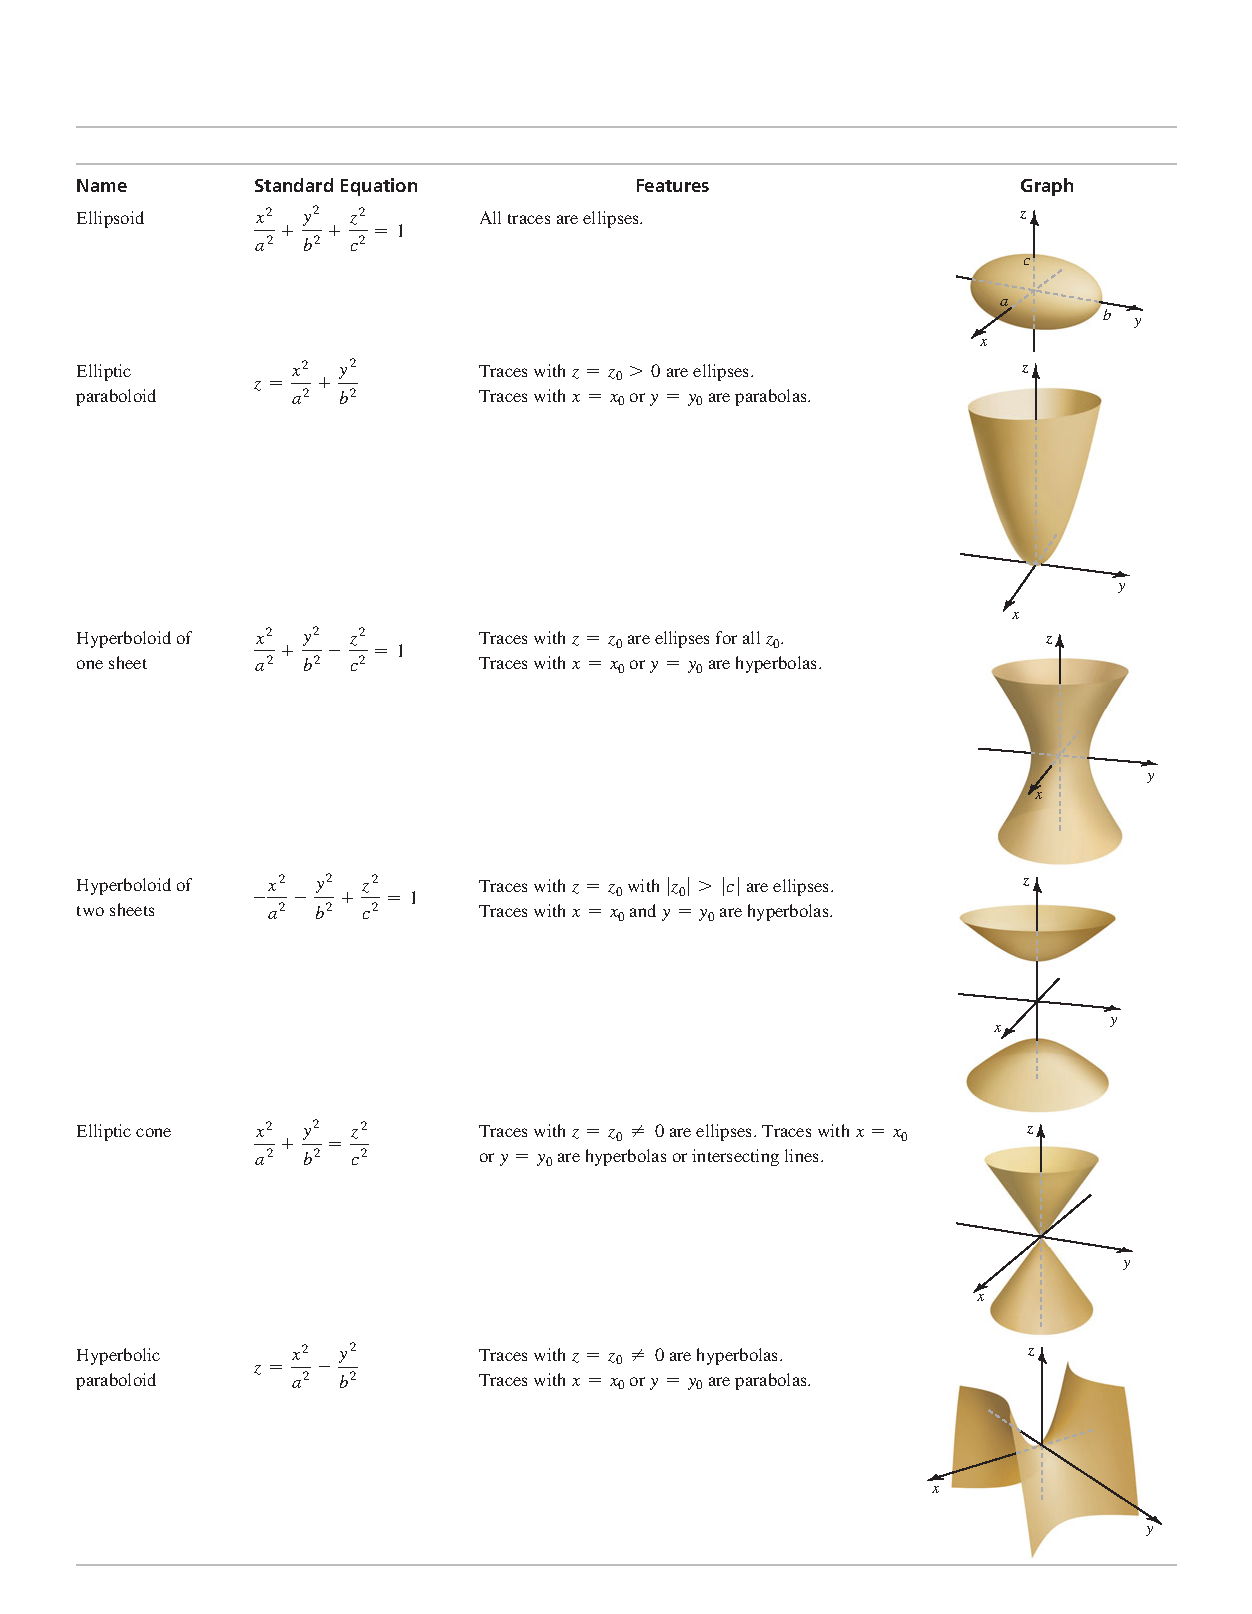
\includepdf{assets/planes-and-surfaces}

\subsection{Graphs and Level Curves}
\subsubsection{Function, Domain, and Range with Two Independent Variables}
A \textbf{function} $z = f(x,\, y)$ assigns to each point $(x,\, y)$ in a set $D$ in $\mathbb{R}^2$ a unique real number $z$ in a subset of $\mathbb{R}$. The set $D$ is the \textbf{domain} of $f$. The \textbf{range} of $f$ is the set of real numbers $z$ that are assumed as the points $(x,\, y)$ vary over the domain.

\subsubsection{Function, Domain, and Range with $\mathbf{n}$ Independent Variables}
The \textbf{function} $y = f(x_1,\, x_2,\, \ldots,\, x_n)$ assigns a unique real number $y$ to each point $(x_1,\, x_2,\, \ldots,\, x_n)$ in a set $D$ in $\mathbb{R}^n$. The set $D$ is the \textbf{domain} of $f$. The \textbf{range} is the set of real numbers $y$ that are assumed as the points $(x_1,\, x_2,\, \ldots,\, x_n)$ vary over the domain.

\subsection{Limits and Continuity}
\subsubsection{Limit of a Function of Two Variables}
The function $f$ has the \textbf{limit} $L$ as $P(x,\, y)$ approaches $P_0(a,\, b)$ written

\begin{equation}
    \lim{(x,\, y) \rightarrow (a,\, b)} f(x,\, y) = \lim{P \rightarrow P_0} f(x,\, y) = L
\end{equation}

if, given any $\varepsilon > 0$, there exists a $\delta > 0$ such that

\begin{equation}
    |f(x,\, y) - L| < \varepsilon
\end{equation}

whenever $(x,\, y)$ is in the domain of $f$ and

\begin{equation}
    0 < |PP_0| = \sqrt{(x - a)^2 + (y - b)^2} < \delta
\end{equation}

\subsubsection{Limits of Constant and Linear Functions}
Let $a, b,$ and $c$ be real numbers.

\begin{enumerate}
    \item Constant functions $f(x,\, y) = c: \limit{(x,\, y) \rightarrow (a,\, b)} c = c$
    \item Linear function $f(x,\, y) = x: \limit{(x,\, y) \rightarrow (a,\, b)} x = a$
    \item Linear function $f(x,\, y) = y: \limit{(x,\, y) \rightarrow (a,\, b)} y = b$
\end{enumerate}

\subsubsection{Limit Laws and Functions of Two Variables}
Let $L$ and $M$ be real numbers and suppose that $\limit{(x,\, y) \rightarrow (a,\, b)} f(x,\, y) = L$ and $\limit{(x,\, y) \rightarrow (a,\, b)} g(x,\, y) = M$. Assume $c$ is a constant, and $\forall m, n \in \mathbb{Z}$.

\begin{enumdescript}
    \item [Sum] $\limit{(x,\, y) \rightarrow (a,\, b)} (f(x,\, y) + g(x,\, y)) = L + M$
    \item [Difference] $\limit{(x,\, y) \rightarrow (a,\, b)} (f(x,\, y) - g(x,\, y)) = L - M$
    \item [Constant multiple] $\limit{(x,\, y) \rightarrow (a,\, b)} cf(x,\, y)  = cL$
    \item [Product] $\limit{(x,\, y) \rightarrow (a,\, b)} f(x,\, y) \cdot g(x,\, y) = L \cdot M$
    \item [Quotient] $\limit{(x,\, y) \rightarrow (a,\, b)} \bigg[ \frac{f(x,\, y)}{g(x,\, y)} \bigg] = \frac{L}{M}$
    \item [Power] $\limit{(x,\, y) \rightarrow (a,\, b)} (f(x,\, y))^n = L^n$
    \item [$\nicefrac{m}{n}$ Power] If $m$ and $n$ have no common factors and $n \neq 0$, then $\limit{(x,\, y) \rightarrow (a,\, b)} [f(x,\, y)]^{\nicefrac{m}{n}} = L^{\nicefrac{m}{n}}$, where we assume $L > 0$ if $n$ is even.
\end{enumdescript}

\subsubsection{Interior and Boundary Points}
Let $R$ be a region in $\mathbb{R}^2$. An \textbf{interior point} $P$ of $R$ lies entirely within $R$, which means it is possible to find a disk centered at $P$ that contains only points of $R$.

A \textbf{boundary point} $Q$ of $R$ lies on the edge of $R$ in the sense that \textit{every} disk centered at $Q$ contains at least one point in $R$ and at least one point not in $R$.

\subsubsection{Open and Closed Sets}
A region is \textbf{open} if it consists entirely of interior points. A region is \textbf{closed} if it contains all its boundary points.

\subsubsection{Two-Path Test for Nonexistence of Limits}
If $f(x,\, y)$ approaches two different values as $(x,\, y)$ approaches $(a,\, b)$ along two different paths in the domain of $f$, then $\limit{(x,\, y)
\rightarrow (a,\, b)} f(x,\, y)$ does not exist.

\subsubsection{Continuity}
A function $f$ is continuous at the point $(a,\, b)$ provided

\begin{enumerate}
    \item $f$ is defined at $(a,\, b)$.
    \item $\limit{(x,\, y) \rightarrow (a,\, b)} f(x,\, y)$ exists.
    \item $\limit{(x,\, y) \rightarrow (a,\, b)} f(x,\, y) = f(a,\, b)$.
\end{enumerate}

\subsubsection{Continuity of Composite Functions}
If $u = g(x,\, y)$ is continuous at $(a,\, b)$ and $z = f(u)$ is continuous at $g(a,\, b)$, then the composite function $z = f(g(x,\, y))$ is continuous at $(a,\, b)$.

\subsection{Partial Derivatives}
The \textbf{partial derivative of $f$ with respect to $x$ at the point (a, b)} is

\begin{equation}
    f_x (a, b) = \lim _{h \rightarrow 0} \frac{f(a + h, b) - f(a, b)}{h}.
\end{equation}

The \textbf{partial derivative of $f$ with respect to $y$ at the point (a, b)} is

\begin{equation}
    f_y (a, b) = \lim _{h \rightarrow 0} \frac{f(a, b + h) - f(a, b)}{h}.
\end{equation}

provided these limits exists.

\subsubsection{Equality of Mixed Partial Derivatives}
Assume that $f$ is defined on an open set $D$ of $\mathbb{R}^2$, and $f_{xy}$ and $f_{yx}$ are continuous throughout $D$. Then $f_{xy} = f_{yx}$ at all points of $D$.

\subsubsection{Differentiability}
The function $z = f(x,\, y)$ is \textbf{differentiable at $(a,\, b)$} provided $f_x(a,\, b)$ and $f_y(a,\, b)$ exist and the change $\Delta z = f(a + \Delta x,\, b + \Delta y) - f(a,\, b)$ equals

\begin{equation}
     \Delta z = f_x (a,\, b) \Delta x + f_y (a,\, b) \Delta y + \varepsilon_1 \Delta x + \varepsilon_2 \Delta y,
\end{equation}

where for fixed $a$ and $b$, $\varepsilon_1$ and $\varepsilon_2$ are functions that depend only on $\Delta x$ and $\Delta y$, with $(\varepsilon_1, \varepsilon_2) \rightarrow (0,\, 0)$ as $(\Delta x,\, \Delta y) \rightarrow (0,\, 0)$. A function is \textbf{differentiable} on an open set $R$ if it is differentiable at every point on $R$.

\subsubsection{Conditions for Differentiability}
Suppose the function $f$ has partial derivatives $f_x$ and $f_y$ defined on an open set containing $(a,\, b)$, with $f_x$ and $f_y$ continuous $(a,\, b)$. Then $f$ is differentiable at $(a,\, b)$.

\subsubsection{Differentiability Implies Continuity}
If a function $f$ is differentiable at $(a,\, b)$, then it is continuous at $(a,\, b)$


\subsection{The Chain Rule}

\subsubsection{Chain Rule (One Independent Variable)}
Let $z$ be a differentiable function of $x$ and $y$ on its domain, where $x$ and $y$ are differentiable functions of $t$ on an interval $I$. Then

\begin{equation}
    \frac{dz}{dt} = \frac{\partial z}{\partial x} \frac{dx}{dt} + \frac{\partial z}{\partial y} \frac{dy}{dt}.
\end{equation}

\subsubsection{Chain Rule (Two Independent Variables)}
Let $z$ be a differentiable function of $x$ and $y$, where $x$ and $y$ are differentiable functions of $s$ and $t$. Then

\begin{equation}
    \frac{dz}{ds} = \frac{\partial z}{\partial x} \frac{\partial x}{\partial s} + \frac{\partial z}{\partial y} \frac{\partial y}{\partial s} \quad \text{and} \quad
    \frac{dz}{dt} = \frac{\partial z}{\partial x} \frac{\partial x}{\partial t} + \frac{\partial z}{\partial y} \frac{\partial y}{\partial t}
\end{equation}

\begin{multicols}{2}
\begin{forest}
for tree={ l sep=40pt,s sep=40pt,}
[z
    [x, edge=red, edge label={node[midway,left] {$\frac{\partial z}{\partial x}$}}
        [s, edge=red, edge label={node[midway,left] {$\frac{\partial x}{\partial s}$}}]
        [t, edge label={node[midway,left] {$\frac{\partial x}{\partial t}$}}]
    ]
    [y, edge=red, edge label={node[midway,left] {$\frac{\partial z}{\partial y}$}}
        [s, edge=red, edge label={node[midway,left] {$\frac{\partial y}{\partial s}$}}]
        [t, edge label={node[midway,left] {$\frac{\partial y}{\partial t}$}}]
    ]
]
\end{forest}

\begin{forest}
for tree={ l sep=40pt,s sep=40pt,}
[z
    [x, edge=red, edge label={node[midway,left] {$\frac{\partial z}{\partial x}$}}
        [s, edge label={node[midway,left] {$\frac{\partial x}{\partial s}$}}]
        [t, edge=red, edge label={node[midway,left] {$\frac{\partial x}{\partial t}$}}]
    ]
    [y, edge=red, edge label={node[midway,left] {$\frac{\partial z}{\partial y}$}}
        [s, edge label={node[midway,left] {$\frac{\partial y}{\partial s}$}}]
        [t, edge=red, edge label={node[midway,left] {$\frac{\partial y}{\partial t}$}}]
    ]
]
\end{forest}
\end{multicols}

\subsubsection{Implicit Differentiation}
Let $F$ be differentiable on its domain and suppose that $F(x,\, y) = 0$ defines $y$ as a differentiable function of $x$. Provided $F_y \neq 0$.

\begin{equation}
    \frac{dy}{dx} = - \frac{F_x}{F_y}
\end{equation}

\subsection{Directional Derivatives and the Gradient}
\subsubsection{Directional Derivative}
Let $f$ be a differentiable at $(a,\, b)$ and let $\textbf{u} = \langle \cos \theta,\, \sin \theta \rangle$ be a unit vector in the $xy$-plane. The \textbf{directional derivatives of $f$ at $(a,\, b)$} in the direction of $\textbf{u}$ is

\begin{equation}
    D _u f(a,\, b) = \lim _{h \rightarrow 0} \frac{f(a + h\cos \theta,\, b + h \sin \theta) - f (a,\, b)}{h}
\end{equation}

provided the limit exits.

\subsubsection{Directional Derivative}
Let $f$ be differentiable on $(a,\, b)$ and let $\textbf{u} = \langle u_1,\, u_2 \rangle$ be a unit vecor in the $x,\, y$-plane. The \textbf{directional derivative of $f$ at a $(a,\, b)$ in the direction of $u$} is

\begin{equation}
    D_u f(a,\, b) = \langle f_x (a,\, b),\, f_y (a,\, b) \rangle \cdot \langle u_1,\, u_2 \rangle
\end{equation}

\subsubsection{Gradient (Two Dimensions)}
Let $f$ be differentiable at the point $(x,\, y)$. The \textbf{gradient} of $f$ at $(x,\, y)$ is the vector-valued function

\begin{equation}
    \nabla f(x,\, y) = \langle f_x (x,\, y),\, f_y (x,\, y) \rangle = f_x (x,\, y) \ihat + f_y (x,\, y) \jhat
\end{equation}

\subsubsection{Directions of Change}
Let $f$ be differentiable at $(a,\, b)$ with $\nabla f(a,\, b) \neq \mathbf{0}$

\begin{enumerate}
    \item $f$ has its maximum rate of increase at $(a,\, b)$ in the direction of the gradient $\nabla f (a,\, b)$. The rate of increase in this direction is $|\nabla f(a,\, b)|$
    \item $f$ has its maximum rate of decrease at $(a,\, b)$ in the direction of $-\nabla f(a,\, b)$. The rate of decrease in this direction is $-|\nabla f(a,\, b)|$.
    \item The directional derivative is zero in any direction orthogonal to $\nabla f (a,\, b)$.
\end{enumerate}

\subsubsection{The Gradient and Level Curves}
Given a function $f$ differentiable at $(a,\, b)$, the line tangent to the level curve of $f$ at $(a,\, b)$ is orthogonal to the gradient $\nabla f(a,\, b)$, provided $\nabla f(a,\, b) \neq \mathbf{0}$.

\subsubsection{Gradient and Directional Derivative in Three Dimensions}
Let $f$ be differentiable at the point $(x,\, y,\, z)$. The \textbf{gradient} of $f$ at $(x,\, y,\, z)$ is the vector-valued function

\begin{align}
    \nabla f(x,\, y,\, z) &= \langle f_x (x,\, y,\, z),\, f_y (x,\, y,\, z),\, f_z (x,\, y,\, z) \rangle \\
    &= f_x (x,\, y,\, z)\ihat + f_y (x,\, y,\, z)\jhat + f_z (x,\, y,\, z)\khat
\end{align}

The \textbf{directional derivative} of $f$ in the direction of the unit vector $\mathbf{u} = \langle u_1,\, u_2,\, u_3 \rangle$ at the point $(a,\, b,\, c)$ is $D_u f(a,\, b,\, c) = \nabla f(a,\, b,\, c) \cdot \mathbf{u}$

\subsection{Tangent Planes and Linear Approximation}
Let $F$ be differentiable at the point $P_0 (a,\, b,\, c)$ with $\nabla F(a,\, b,\, c) \neq \mathbf{0}$. The plane tangent to the surface $F(x,\, y,\, z) = 0$ at $P_0$, called the \textbf{tangent plane}, is the plane passing through $P_0$ orthogonal $\nabla F(a,\, b,\, c)$. An equation of the tangent plane is

\begin{equation}
    F_x (a,\, b,\, c)(x - a) + F_y (a,\, b,\, c)(y - b) + F_z (a,\, b,\, c)(z - c) = 0.
\end{equation}

\subsubsection{Tangent Plane for $z = f(x,\, y)$}
Let $f$ be differentiable at the point $(a,\, b)$. An equation of the plane tangent to the surface $z = f(x,\, y)$ at the point $(a,\, b,\, f(a,\, b))$ is

\begin{equation}
    z = f_x (a,\, b)(x - a) + f_y (a,\, b)(y - b) + f(a,\, b)
\end{equation}

\subsubsection{Linear Approximation}
Let $f$ be differentiable at $(a,\, b)$. The linear approximation to the surface $z = f(x,\, y)$ at the point $(a,\, b,\, f(a,\, b))$ is the tangent plane at that point, given by the equation

\begin{equation}
    L(x,\, y) = f_x (a,\, b)(x - a) + f_y (a,\, b)(y - b) + f(a,\, b)
\end{equation}

\subsubsection{The Differential $dz$}
Let $f$ be differentiable at the point $(a,\, b)$. The change in $z = f(x,\, y)$ as the independent variables change from $(a,\, b)$ to $(a + dx,\, b + dy)$ is denoted by the differential $dz$:

\begin{equation}
    \Delta z \approx dz = f_x(a,\, b) dx + f_y(a,\, b) dy
\end{equation}

\subsection{Maximum/Minimum Problems}
\subsubsection{Local Maximum/Minimum Values}
A function $f$ has a \textbf{local maximum value} at $(a, b)$ if $f(x, y) \leq f(a, b)$ for all $(x, y)$ in the domain of $f$ in some open disk centered at $(a, b)$. A function $f$ has a \textbf{local minimum value} at $(a, b)$ if $f(x, y) \geq f(a, b)$ for all $(x, y)$ in the domain of $f$ in some open disk centered at $(a, b)$. Local maximum and local minimum values are also called \textbf{local extreme values} or \textbf{local extrema}.

\subsubsection{Derivatives and Local Maximum/Minimum Values}
If $f$ has a local maximum or minimum value at $(a, b)$ and the partial derivatives $f_x$ and $f_y$ exist at $(a, b)$ then $f_x (a, b) = f_y(a, b) = 0$.

\subsubsection{Critical Point}
An interior point $(a,\, b)$ in the domain of $f$ is a \textbf{critical point} of $f$ is either

\begin{enumerate}
    \item $f_x (a,\, b) = f_y (a,\, b) = 0$, or
    \item one (or both) of $f_x$ or $f_y$ does not exist at $(a,\, b)$
\end{enumerate}

\subsubsection{Saddle Point}
A function $f$ has a \textbf{saddle point} at a critical point $(a,\, b)$ if, in every open disk centered at $(a,\, b)$, there are points $(x,\, y)$ for which $f(x,\, y) > f(a,\, b)$ and points for which $f(x,\, y) < f(a,\, b)$

\subsubsection{Second Derivative Test}
Suppose that the second partial derivative of $f$ are continuous throughout an open disk centered at the point $(a,\, b)$, where $f_x (a,\, b) = f_y (a,\, b) = 0$. Let $D(x,\, y) = f_{xx} (x,\, y) f_{yy} (x,\, y) - (f_{xy} (x,\, y))^2$.

\begin{enumerate}
    \item If $D(a,\, b) > 0$ and $f_{xx} (a,\, b) < 0$, then $f$ has a local maximum value at $(a,\, b)$.
    \item If $D(a,\, b) > 0$ and $f_{xx} (a,\, b) > 0$, then $f$ has a local minimum value at $(a,\, b)$.
    \item If $D(a,\, b) < 0$, then $f$ has a saddle point at $(a,\, b)$.
    \item If $D(a,\, b) = 0$, then the test is inconclusive.
\end{enumerate}

\subsubsection{Absolute Maximum/Minimum Values}
If $f(x,\, y) \leq f(a,\, b)$ for all $(x,\, y)$ in the domain of $f$, then $f$ has an \textbf{absolute maximum value} at $(a,\, b)$. If $f(x,\, y) \geq f(a,\, b)$ for all $(x,\, y)$ in the domain of $f$, then $f$ has an \textbf{absolute minimum value} at $(a,\, b)$.

\subsubsection{Finding Absolute Maximum/Minimum Values on Closed, Bounded Sets}
Let $f$ be continuous on a closed bounded set $R$ in $\mathbb{R}^2$. To find the absolute maximum and minimum values of $f$ on $R$:

\begin{enumerate}
    \item Determine the values of $f$ at all critical points in $R$.
    \item Find the maximum and minimum values of $f$ on the boundary of $R$.
    \item The greatest function values found in Step 1 and 2 is the absolute maximum value of $f$ on $R$, and the least function value found in Steps 1 and 2 is the absolute minimum value of $f$ on $R$.
\end{enumerate}

\subsection{Lagrange Multipliers}
\subsubsection{Parallel Gradients (Ball Park Theorem)}
Let $f$ be a differentiable function in a region of $\mathbb{R}^2$ that contains the smooth curve $C$ given by $g(x, y) = 0$. Assume that $f$ has a local extreme value (relative to values of $f$ on $C$) at a point $P(a, b)$ on $C$. Then $\nabla f(a, b)$ is orthogonal to the line tangent to $C$ at $P$. Assuming $\nabla g(a, b) \neq 0$, it follows that there is a real number $\lambda$ (called a \textbf{Lagrange multiplier}) such that $\nabla f(a, b) = \lambda \nabla g(a, b)$.

\subsubsection{Method of Lagrange Multipliers in Two Variables}
Let the objective function $f$ and the constraint function $g$ be differentiable on a region of $\mathbb{R}^2$ with $\lambda g(x, y) \neq 0$ on the curve $g(x, y) = 0$. To locate the maximum and minimum values of $f$ subject to the constraint $g(x, y) = 0$, carry out the following steps.

\begin{enumerate}
    \item Find the values of $x, y$ and $\lambda$ (if they exist) that satisfy the equations

    \begin{equation}
        \nabla f(x,\, y) = \lambda \nabla g(x,\, y) \quad \text{and} \quad g(x,\, y) = 0
    \end{equation}

    \item Among the values $(x,\, y)$ found in Step 1, select the largest and smallest corresponding function values, which are the maximum and minimum values of $f$ subject to the constraint.
\end{enumerate}

\subsubsection{Method of Lagrange Multipliers in Three Variables}
Let $f$ and $g$ be differentiable on a region of $\mathbb{R}^3$ with $\nabla g(x,\, y,\, z) neq 0$ on the surface $g(x,\, y,\, z) = 0$. To locate the maximum and minimum values of $f$ subject to the constraint $g(x,\, y,\, z) = 0$, carry out the following steps.

\begin{enumerate}
    \item Find the values of $x,\, y,\, z$ and $\lambda$ that satisfy the equations

    \begin{equation}
        \nabla f(x,\, y,\, z) = \lambda \nabla g(x,\, y,\, z) \quad \text{and} \quad g(x,\, y,\, z) = 0
    \end{equation}

    \item Among the points $(x,\, y,\, z)$ found in Step 1, select the largest and smallest corresponding values of the objective function. These values are the maximum and minimum values of $f$ subject to the constraint.
\end{enumerate}


\section{Multiple Integration}
\subsection{Double Integrals over Rectangular Regions}
\subsubsection{Volumes and Double Integrals}
A function $f$ defined on a rectangular region $R$ in the $xy$-plane is \textbf{integratabtle} on $R$ if $\limit{\Delta \rightarrow 0} \sum _{k = 1} ^{n} f(x_k ^*, y_k ^*) \Delta A_k$ exists fora ll partitions of $R$ and for all choices of $(x_k ^*,\, y_k ^*)$ within those partitions. The limit is the \textbf{double integral of $f$ over $R$}, which we write

\begin{equation}
    \iint \limits _R f(x,\, y) \,dA = \limit{\Delta \rightarrow 0} \sum _{k = 1} ^{n} f(x_k ^*,\, y_k ^*) \Delta A_k
\end{equation}

If $f$ is nonnegative on $R$, then the double integral equals the volume of the solid bounded by $z = f(x,\, y)$ and the $xy$-plane over $R$.

\subsubsection{Double Integrals on Rectangular Regions}
Let $f$ be continuous on the rectangular region $R = \{ (x,\, y): a \leq x \leq b,\, c \leq y \leq d \}$. The double integral of $f$ over $R$ may be evaluated by either of two iterated integrals:

\begin{equation}
    \iint \limits _R f(x,\, y) \,dA = \int _c ^d \int _a ^b dx\,dy = \int _a ^b \int _c ^d dy\,dx
\end{equation}

\subsubsection{Average Value of a Function over a Plane Region}
The \textbf{average value} of an integrable function $f$ over a region $R$ is

\begin{equation}
    \bar{f} = \frac{1}{\text{area of}\ R} \iint \limits _R f(x,\, y)\, dA
\end{equation}

\subsection{Double Integrals over General Regions}
Let $R$ be a region bounded below and above by the graphs of the continuous functions $y = g(x)$ and $y = h(x)$, respectively, and by the lines $x = a$ and $x = b$. If $f$ is continuous on $R$, then

\begin{equation}
    \iint \limits _R f(x, y) \,dA = \int _a ^b \int _{g(x)} ^{h(x)} f(x, y)\, dy\, dx
\end{equation}

Let $R$ be a region bounded on the left and right by the graphs of the continuous functions $x = g(y)$  and $x = h(y)$, respectively, and the lines $y = c$ and $y = d$. If $f$ is continuous on $R$, then

\begin{equation}
    \iint \limits _R f(x,\, y) \,dA = \int _c ^d \int _{g(y)} ^{h(y)} f(x,\, y)\, dx\, dy
\end{equation}

\subsubsection{Areas of Regions by Double Integrals}
Let $R$ be a region in the $xy$-plane. Then

\begin{equation}
    \text{area of}\ R = \iint \limits _R
\end{equation}

\subsection{Double Integrals in Polar Coordinates}
\subsubsection{Double Integrals over Polar Rectangular Region}
Let $f$ be continuous on the region in the $xy$-plane $R = \{ (r, \theta): 0 \leq a \leq r \leq b, \alpha \leq \theta \leq \beta \}$, where $\beta - \alpha \leq 2\pi$. Then

\begin{equation}
    \iint \limits _R f(r, \theta) \, dA = \int _\alpha ^\beta \int _a ^b f(r, \theta) \ r \,dr\,d\theta
\end{equation}

\subsubsection{Double Integrals over More General Polar Regions}
Let $f$ be continuous on the region in the $xy$-plane

\begin{equation}
    R = \{ (r, \theta): 0 \leq g(\theta) \leq r \leq h(\theta), \alpha \leq \theta \leq \beta \}
\end{equation}

where $0 < \beta - \alpha \leq 2\pi$. Then

\begin{equation}
    \iint \limits _R f(r, \theta) \,dA = \int _\alpha ^\beta \int _{g(\theta)} ^{h(\theta)} f(r, \theta) r \,dr\,d\theta.
\end{equation}

\subsubsection{Area of Polar Regions}
The area of the region $R = \{ (r, \theta): 0 \leq g(\theta) \leq r \leq h(\theta), \alpha \leq \theta \leq \beta \}$, where $0 < \beta - \alpha \leq 2\pi$, is

\begin{equation}
    A = \iint \limits _R \, dA = \int _\alpha ^\beta \int _{g(\theta)} ^{h(\theta)} \ r \,dr\,d\theta
\end{equation}

\subsection{Triple Integrals}
Let $f$ be continuous over the region

\begin{equation}
    D = \{ (x,\, y,\, z): a \leq x \leq b, g(x) \leq y \leq h(x),\, G(x,\, y) \leq z \leq H(x,\, y) \}
\end{equation}

where $g, h, G,$ and $H$ are continuous functions. Then $f$ is integrable over $D$ and the triple integral is evaluated as the iterated integral

\begin{equation}
    \iiint \limits _D f(x,\, y,\, z) \,dV = \int _a ^b \int _{g(x)} ^{h(x)} \int _{G(x,\, y)} ^{H(x,\, y)} f(x,\, y,\, z) \,dz\,dy\,dx.
\end{equation}

\subsubsection{Average Value of a Function of Three Variables}
If $f$ is continuous on a region $D$ of $\mathbb{R}^3$, then the average value of over $D$ is

\begin{equation}
    \bar{f} = \frac{1}{\text{volume}\ (D)} \iiint \limits _D f(x,\, y,\, z) \,dV
\end{equation}

\subsection{Triple Integrals in Cylindrical and Spherical Coordinates}
\subsubsection{Transformations Between Cylindrical and Rectangular Coordinates}

\begin{center}
    \begin{tabular}{cc}
        \textbf{Rectangular \textrightarrow \ Cylindrical} & \textbf{Cylindrical \textrightarrow \ Rectangular} \\
        $r^2 = x^2 + y^2$ & $x = r \cos\theta$ \\
        $\tan\theta = \nicefrac{y}{x}$ & $y = r \sin\theta$ \\
        $z = z$ & $z = z$ \\
    \end{tabular}
\end{center}

\subsubsection{Triple Integrals in Cylindrical Coordinates}
Let $f$ be continuous over the region

\begin{equation}
    D = \{ (r,\, \theta,\, z): g(\theta) \leq r \leq h(\theta),\, \alpha \leq \theta \leq \beta,\, G(x,\, y) \leq z \leq H(x,\, y). \}
\end{equation}

Then $f$ is integrable over $D$ and the triple integral of $f$ over $D$ in cylindrical coordinates is

\begin{equation}
    \iiint \limits _D f(r,\, \theta,\, z) \,dV = \int _\alpha ^\beta \int _{g(\theta)} ^{h(\theta)} \int _{G(r \cos\theta,\, r\sin\theta)} ^{H(r \cos\theta,\, r\sin\theta)} f(r,\, \theta,\, z) \,dz \ r \,dr \,d\theta
\end{equation}

\subsubsection{Tranformations Between Spherical and Rectangular Coordinates}
\begin{center}
    \begin{tabular}{cc}
        \textbf{Rectangular \textrightarrow \ Spherical} & \textbf{Spherical \textrightarrow \ Rectangular} \\
        $\rho^2 = x^2 + y^2 + z^2$ & $x = \rho \sin \varphi \cos \theta$ \\
        Use trigonometry to find $\varphi$ and $\theta$ & $y = \rho \sin \varphi \sin \theta$ \\
        & $z = \rho \cos \varphi$\\
    \end{tabular}
\end{center}

\subsubsection{Triple Integrals in Spherical Coordinates}
Let $f$ be continuous over the region

\begin{equation}
    D = \{ (\rho,\, \varphi,\, \theta): g(\varphi,\, \theta) \leq \rho \leq h(\varphi,\, \theta),\, a \leq \varphi b,\, \alpha \leq \theta \leq \beta \}
\end{equation}

Then $f$ is integrable over $D$, and the triple integral of $f$ over $D$ in spherical coordinates is

\begin{equation}
    \iiint \limits _D \, f(\rho,\, \varphi,\, \theta) dV = \int _\alpha ^\beta \int _a ^b \int _{g(\varphi,\, \theta)} ^{h(\varphi,\, \theta)} f(\rho,\, \varphi,\, \theta) \rho^2 \sin \varphi \ d\rho\, d\varphi\, d\theta
\end{equation}

\subsection{Integrals for Mass Calculations}
\subsubsection{Center of Mass in One Dimension}
Let $\rho$ be an integrable density function on the interval $[a,\, b]$ (which represents a thin rod or wire). The \textbf{center of mass} is location at the point $\bar{x} = \frac{M}{m}$, where the \textbf{total moment} $M$ and mass $m$ are

\begin{equation}
    M = \int _a ^b x\rho(x) \, dx \quad \text{and} \quad m = \int _a ^b \rho(x)\, dx
\end{equation}

\subsubsection{Center of Mass in Two Dimensions}
Let $\rho$ be integrable density function defined over a closed bounded region $R$ in $\mathbb{R}^2$. The coordinates of the center of mass of the object represented by $R$ are

\begin{equation}
    \bar{x} = \frac{M_y}{m} = \frac{1}{m} \iint \limits _R x\rho(x,\, y)\, dA \quad \text{and} \quad \bar{y} = \frac{M_x}{m} = \frac{1}{m} = \iint \limits _R y \rho(x,\, y)\, dA
\end{equation}

\subsubsection{Center of Mass in Three Dimensions}
Let $\rho$ be integrable density function on a closed bounded region $D$ in $\mathbb{R}^3$. The coordinates of the center of mass of the region are

\begin{align}
    \bar{x} &= \frac{M_{yz}}{m} = \frac{1}{m} \iiint \limits _R x\rho(x,\, y,\, z)\, dV \\
    \bar{y} &= \frac{M_{xz}}{m} = \frac{1}{m} \iiint \limits _R y\rho(x,\, y,\, z)\, dV \\
    \bar{z} &= \frac{M_{xy}}{m} = \frac{1}{m} \iiint \limits _R z\rho(x,\, y,\, z)\, dV
\end{align}

where $m = \iiint _D \rho(x,\, y,\, z)\, dV$ is the mass, and $M_{yz},\, M_{xz}$ and $M_{xy}$ are the moments with respect to the coordinate planes.


\section{Vector Calculus}
\subsection{Vector Fields}
\subsubsection{Vector Fields in Two Dimensions}
Let $f$ and $g$ be defined on a region $R$ of $\mathbb{R}^2$. A \textbf{vector field} in $\mathbb{R}^2$ is a function $\mathbf{F}$ that assigns to each point in $R$ a vector $\langle f(x, y),\, g(x, y) \rangle$. The vector field is written as

\begin{equation}
    \mathbf{F}(x, y) = \langle f(x, y),\, g(x, y) \rangle \quad\text{or}\quad \mathbf{F}(x, y) = f(x, y) \ihat + g(x, y) \jhat
\end{equation}

A vector field $\mathbf{F} = \langle f, g \rangle$ is continuous or differentiable on a region $R$ of $\mathbb{R}^2$ if $f$ and $g$ are continuous or differentiable on $R$, respectively.

\subsubsection{Radial Vector Fields in $\mathbb{R}^2$}
Let $\mathbf{r} = \langle x,\, y \rangle$. A vector field of the form $\mathbf{F} = f(x,\, y) \mathbf{r}$, where $f$ is a scalar-valued function, is a \textbf{radial vector field}. Of specific interest are the radial vector field

\begin{equation}
    \mathbf{F}(x,\, y) = \frac{\mathbf{r}}{|\mathbf{r}|^p} = \frac{\langle x,\, y \rangle}{|\mathbf{r}|^p}
\end{equation}

where $p$ is a real number. At every point (except the origin), the vectors of this field are directed outward from the origin with the magnitude of $|\mathbf{F}| = \frac{1}{|\mathbf{r}|^{p - 1}}$.

\subsubsection{Vector Fields in Three Dimensions}
Let $f$,\, $g$,\, and $h$ be defined on a region $D$ of $\mathbb{R}^3$. A \textbf{vector field} in $\mathbb{R}^3$ is a function $\mathbf{F}$ that assigns to each point in $D$ a vector $\langle f(x,\, y,\, z),\, g(x,\, y,\, z),\, h(x,\, y,\, z) \rangle$. The vector field is written as

\begin{align}
    &\mathbf{F}(x,\, y,\, z) = \langle f(x,\, y,\, z),\, g(x,\, y,\, z),\,  h(x,\, y,\, z) \rangle \quad\text{or}\\
    &\mathbf{F}(x,\, y,\, z) =  f(x,\, y,\, z)\ihat +  g(x,\, y,\, z)\jhat + h(x,\, y,\, z)\khat
\end{align}

A vector field $\mathbf{F} = \langle f,\, g,\, h \rangle$ is continuous or differentiable on a region $D$ of $\mathbb{R}^3$ if $f$,\, $g$,\, $h$ are continuous or differentiable on $R$, respectively. Of particular importance are the \textbf{radial vector fields}

\begin{equation}
    \mathbf{F}(x,\, y,\, z) = \frac{\mathbf{r}}{|\mathbf{r}|^p} = \frac{\langle x,\, y,\, z \rangle}{|\mathbf{r}|^p}
\end{equation}

where $p$ is a real number.

\subsubsection{Gradient Fields and Potential Functions}
Let $z = \varphi(x,\, y)$ and $w = \varphi(x,\, y,\, z)$ be differentiable functions on regions of $\mathbb{R}^2$ and $\mathbb{R}^3$, respectively. The vector field $\mathbf{F} = \nabla \varphi$ is \textbf{gradient field}, and the function $\varphi$ is a \textbf{potential function} for \textbf{F}.

\subsection{Line Integrals}
\subsubsection{Scalar Line Integral in the Plane, Arc Length Parameter}
Suppose the scalar-valued function $f$ is defined on the smooth curve $C: \mathbf{r}(s) = \langle x(s),\, y(s) \rangle$, parameterized by the arc length $s$. The \textbf{line integral of $f$ over $C$} is

\begin{equation}
    \int \limits _C f(x(s) ,\, y(s)) \, ds = \lim _{\Delta \rightarrow 0} \sum _{k = 1} ^{n} f(x(s_k ^*),\, y(s_k ^*)) \Delta s_k,
\end{equation}

provided this limit exists over all partitions of $C$. When the limit exists, $f$ is said to be \textbf{integrable} on $C$.

\subsubsection{Evaluating Scalar Line Integrals in $\mathbb{R}^2$}
Let $f$ be continuous on a region containing a smooth curve $C: \mathbf{r}(t) = \langle x(t),\, y(t) \rangle$, for $a \leq t \leq b$. Then

\begin{align}
    \int \limits _C f \, ds &= \int _a ^b f(x(t),\, y(t))|\mathbf{r}'(t)| \, dt \\
    &= \int _a ^b f(x(t),\, y(t))\sqrt{x'(t)^2 + y'(t)^2} \, dt
\end{align}

\subsubsection{Evaluating the Line Integral $\int \limits _C f \, ds$}
\begin{enumerate}
    \item Find a parametric description of $C$ in the form $\mathbf{r}(t) = \langle x(t),\, y(t) \rangle$, for $a \leq t \leq b$
    \item Computer $|\mathbf{r}'(t)| = \sqrt{x'(t)^2 + y'(t)^2}$
    \item Make substitutions for $x$ and $y$ in the integrand and evaluate an ordinary integral

    \begin{equation}
        \int \limits _C f \, ds = \int _a ^b f(x(t),\, y(t)) |\mathbf{r}'(t)| \, dt
    \end{equation}
\end{enumerate}

\subsubsection{Evaluating Scalar Line Integrals in $\mathbb{R}^3$}
Let $f$ be continuous on a region containing a smooth curve $C: \mathbf{r}(t) = \langle x(t),\, y(t),\, z(t) \rangle$, for $a \leq t \leq b$. Then

\begin{align}
    \int f \, ds &= \int _a ^b f(x(t),\, y(t),\, z(t))|\mathbf{r}'(t)| \, dt \\
    &= \int _a ^b f(x(t),\, y(t),\, z(t))\sqrt{x'(t)^2 + y'(t)^2 + z'(t)^2} \, dt
\end{align}

\subsubsection{Line Integral of a Vector Field}
Let $\mathbf{F}$ be a vector field that is continuous on a region containing a smooth oriented curve $C$ parameterized by arc length. Let $\mathbf{T}$ be the unit tangent vector at each point of $C$ consistent with the orientation. The line integral of $\mathbf{F}$ over $C$ is $\int _C \mathbf{F \cdot T} \, ds$.

\subsubsection{Different Forms of Line Integrals of Vector Fields}
The line integral $\int _C \mathbf{F \cdot T} \, ds$ may be expressed in the following forms, where $\mathbf{F} = \langle f,\, g,\, h \rangle$, for $a \leq t \leq b$:

\begin{align}
    \int _a ^b \mathbf{F \cdot r}'(t) \, dt &= \int _a ^b (f\,x'(t),\, g\,y'(t),\, h\,z'(t)) \, dt \\
    &= \int \limits _C f \, dx + g \, dy + h \, dz \\
    &= \int \limits _C \mathbf{F} \cdot  d\mathbf{r}
\end{align}

For line integrals in the plane, we let $\mathbf{F} = \langle f,\, g \rangle$ and assume $C$ is parameterized in the form $\mathbf{r}(t) = \langle x(t),\, y(t) \rangle$, for $a \leq t \leq b$. Then

\begin{equation}
    \int \limits _C \mathbf{F \cdot T} \, ds = \int _a ^b (f \, x'(t) + g \, y'(t)) \, dt = \int \limits _C f \, dx + g \, dy = \int _C \mathbf{F} \cdot d\mathbf{r}
\end{equation}

\subsubsection{Work Done in a Force Field}
Let $\mathbf{F}$ be a continuous force field in a region $D$ of $\mathbb{R}^3$ and let $C: \mathbf{r}(t) = \langle x(t),\, y(t),\, z(t) \rangle$, for $a \leq t \leq b$, be a smooth curve in $D$ with a unit tangent vector $\mathbf{T}$ consistent with the orientation. The work done in moving an object $C$ in the positive direction is

\begin{equation}
    W = \int \limits _C \mathbf{F \cdot T} \, ds = \int _a ^b \mathbf{F \cdot r'(t)} \, dt
\end{equation}

\subsubsection{Circulation}
Let $\mathbf{F}$ be a continuous vector field on a region $D$ of $\mathbb{R}^3$ and let $C$ be a closed smooth oriented curve in $D$. The \textbf{circulation} of $\mathbf{F}$ on $C$ is $\int _C \mathbf{F \cdot T} \, ds$, where $\mathbf{T}$ is the unit vector tangent to $C$ consistent with the orientation.

\subsubsection{Flux}
Let $F = \langle f, g \rangle$ be continuous vector field on a region $R$ of $\mathbb{R}^2$. Let $C: \mathbf{r}(t) = \langle x(t),\, y(t) \rangle$, for $a \leq t \leq b$, be a smooth oriented curve in $R$ that does not intersect itself. The \textbf{flux} of the vector field across $C$ is

\begin{equation}
    \int \limits _C \mathbf{F \cdot n} \, ds = \int _a ^b (f\, y'(t) - g \, x'(t)) \, dt,
\end{equation}

where $n = \mathbf{T} \times \khat$ is the unit normal vector and $\mathbf{T}$ is the unit tangent vector consistent with the orientation. If $C$ is a closed curve with counterclockwise orientation, \textbf{n} is the outward normal vector and the flux integral gives the \textbf{outward flux} across $C$.

\subsection{Conservative Vector Fields}

\subsubsection{Simple and Closed Curves}
Suppose a curve $C$ (in $\mathbb{R}^2$ and $\mathbb{R}^3$) is described parametrically by $\mathbf{r}(t)$, where $a \leq t \leq b$. Then $C$ is a \textbf{simple curve} if $\mathbf{r}(t_1) \neq \mathbf{r}(t_2)$ for all $t_1$ and $t_2$, with $a < t_1 < t_2 < b$; that is, $C$ never intersects itself between its endpoints. The curve $C$ is \textbf{closed} if $\mathbf{r}(a) = \mathbf{r}(b)$; that is, the initial and terminal points of $C$ are the same.

\subsubsection{Connected and Simply Connected Regions}
An open region $R$ in $\mathbb{R}^2$ (or $D$ in $\mathbb{R}^3$) is \textbf{connected} if it possible to connect any two points of $R$ by a continuous curve lying in $R$. An open region $R$ is \textbf{simply connected} if every closed simple curve in $R$ can be deformed and contracted to a point in $R$.

\subsubsection{Conservative Vector Field}
A vector field $F$ is said to be \textbf{conservative} on a region (in $\mathbb{R}^2$ or $\mathbb{R}^3$) if there exists a scalar function $\varphi$ such that $\mathbf{F} = \nabla \varphi$ on that region.

\subsubsection{Test for Conservative Vector Fields}
Let $\mathbf{F} = \langle f,\, g,\, h \rangle$ be a vector field defined on a connected and simply connected region $D$ of $\mathbb{R}^3$, where $f$, $g$, and $h$ have continuous first partial derivatives on $D$. Then $\mathbf{F}$ is a conservative vector field on $D$ (there is a potential function $\varphi$ such that $\mathbf{F} = \nabla \varphi$) if and only if

\begin{equation}
    \frac{\partial f}{\partial y} = \frac{\partial g}{\partial x}, \quad \frac{\partial f}{\partial z} = \frac{\partial h}{\partial x}, \quad\text{and}\quad \frac{\partial g}{\partial z} = \frac{\partial h}{\partial y}
\end{equation}

For vector fields in $\mathbb{R}^2$, we have the single condition $\frac{\partial f}{\partial y} = \frac{\partial g}{\partial x}$.


\subsubsection{Finding Potential Functions in $\mathbb{R}^3$}
Suppose $\mathbf{F} = \langle f,\, g,\, h \rangle$ is a conservative vector field. To find $\varphi$ such that $\mathbf{F} = \nabla \varphi$, take the following steps:

\begin{enumerate}
    \item Integral $\varphi _x = f$ with respect to $x$ to obtain $\varphi$, which includes an arbitrary function $c(y,\, z)$.
    \item Compute $\varphi _y$ and equate it to $g$ to obtain an expression for $c_y (y,\, z)$.
    \item Integrate $c_y (y,\, z)$ with respect to $y$ to obtain $c(y,\, z)$, including an arbitrary function $d(z)$.
    \item Compute $\varphi _z$ and equate it to $h$ to get $d(z)$.
\end{enumerate}

Beginning the procedure with $\varphi _y = g$ or $\varphi _z = h$ maybe be easier in some cases.

\subsubsection{Fundamental Theorem for Line Integrals}
Let $\mathbf{F}$ be a continuous vector field on an open connected region $R$ in $\mathbb{R}^2$ (or $D$ in $\mathbb{R}^3$). There exists a potential function $\varphi$ with $\mathbf{F = \nabla \varphi}$ (which means that $\mathbf{F}$ is conservative) if and only if

\begin{equation}
    \int \limits _C \mathbf{F \cdot T} \, ds = \int \limits _C \mathbf{F} \cdot d\mathbf{r} = \varphi (B) - \varphi(A)
\end{equation}

for all points $A$ and $B$ in $R$ and all smooth oriented curves $C$ from $A$ to $B$.

\subsubsection{Line Integrals on Closed Curves}
Let $R$ in $\mathbb{R}^2$ (or $D$ in $\mathbb{R}^3$) be an open region. Then $\mathbf{F}$ is a conservative vector field on $R$ if and only if $\oint _C \mathbf{F} \cdot d\mathbf{r} = 0$ on all simple closed smooth oriented curves $C$ in $R$.

\subsection{Green's Theorem}
Let $C$ be a simple closed smooth curve, oriented counterclockwise, that encloses a connected and simply connected region $R$ in the plane. Assume $\mathbf{F} = \langle f,\, g \rangle$, where $f$ and $g$ have continuous first partial derivatives in $R$. Then

\begin{equation}
    \oint \limits _C \mathbf{F} \cdot d\mathbf{r} = \oint f \, dx + g \, dy = \iint \limits _R \left( \frac{\partial g}{\partial x} - \frac{\partial f}{\partial y} \right) dA.
\end{equation}

\subsubsection{Two-Dimensional Curl}
The \textbf{two-dimensional curl} of the vector field $\mathbf{F} = \langle f,\, g \rangle$ is $\frac{\partial g}{\partial x} - \frac{\partial f}{\partial y}$. If the curl is zero throughout a region, the vector field is said to be \textbf{irrotational} on that region.

\subsubsection{Area of a Plane Region by Line Integrals}
Under the conditions of Green's Theorem, the area of a region $R$ enclosed by a curve $C$ is

\begin{equation}
    \oint \limits _C x \, dy = - \oint \limits _C y \, dx = \frac{1}{2} \oint \limits _C (x \, dy - y \, dx)
\end{equation}

\subsubsection{Green's Thoerem, Flux Form}
Let $C$ be a simple closed smooth curve, oriented counterclockwise, that encloses a connected and simply connected region $R$ in the plane. Assume $\mathbf{F} = \langle f,\, g \rangle$, where $f$ and $g$ have continuous first partial derivatives in $R$. Then

\begin{equation}
    \oint \limits _C \mathbf{F \cdot n} \, ds = \oint \limits _C f \, dy - g \, dx = \iint \limits _R \left( \frac{\partial f}{\partial x} + \frac{\partial g}{\partial y} \right)
\end{equation}

where $\mathbf{n}$ is the outward unit normal vector on the curve.

\subsubsection{Two-Dimensional Divergence}
The \textbf{two-dimensional divergence} of the vector field $\mathbf{F} = \langle f,\, g \rangle$ is $\frac{\partial f}{\partial x} + \frac{\partial g}{\partial y}$. If the divergence is zero thoughout a region, the vector field is said to be \textbf{source free} on that region.

\subsection{Divergence and Curl}
\subsubsection{Divergence of a Vector Field}
The \textbf{divergence} of a vector field $\mathbf{F} = \langle f,\, g,\, h \rangle$ that is differentiable on a region of $\mathbb{R}^3$ is

\begin{equation}
    \text{div} \, \mathbf{F} = \mathbf{\nabla \cdot F} = \frac{\partial f}{\partial x} + \frac{\partial g}{\partial y} + \frac{\partial h}{\partial z}
\end{equation}

If $\mathbf{\nabla \cdot F} = 0$, the vector field is \textbf{source free.}

\subsubsection{Divergence of Radial Vector Fields}
For a real number $p$, the divergence of the radial vector field

\begin{equation}
    \mathbf{F} = \frac{\mathbf{r}}{|r|^p} = \frac{\langle x,\, y,\, z \rangle}{(x^2 + y^2 + z^2)^\frac{p}{2}} \ \text{is} \ \nabla \cdot \mathbf{F} = \frac{3 - p}{|\mathbf{r}|^p}
\end{equation}

\subsubsection{Curl of a Vector Field}
The \textbf{curl} of a vector field $\mathbf{F} = \langle f,\, g,\, h \rangle$ that is differentiable on a region of $\mathbb{R}^3$ is

\begin{equation}
    \nabla \times \mathbf{F} = \text{curl} \, \mathbf{F} = \left( \frac{\partial h}{\partial y} - \frac{\partial g}{\partial z} \right)\ihat + \left( \frac{\partial f}{\partial z} - \frac{\partial h}{\partial x} \right)\jhat + \left( \frac{\partial g}{\partial x} - \frac{\partial f}{\partial y} \right)\khat
\end{equation}

If $\nabla \times \mathbf{F = 0}$, the vector field is \textbf{irrotational}.

\subsubsection{Curl of a Conservative Vector Field}
The \textbf{general rotation vector field} is $\mathbf{F = a \times r}$, where the nonzero constant vector $\mathbf{a} = \langle a_1,\, a_2,\, a_3 \rangle$ is the axis of ration and $\mathbf{r} = \langle x,\, y,\, z \rangle$. For all nonzero choices of $\mathbf{a}, | \nabla \times \mathbf{F} | = 2|\mathbf{a}|$ and $\mathbf{\nabla \cdot F} = 0$. The constant angular speed of the vector field is

\begin{equation}
    \omega = |\mathbf{a}| = \frac{1}{2}| \nabla \times \mathbf{F} |
\end{equation}

\subsubsection{Curl of a Conservative Vector Field}
Suppose that $\mathbf{F}$ is a conservative vector field on an open region $D$ of $\mathbb{R}^3$. Let $\mathbf{F} = \nabla \varphi$, where $\varphi$ is a potential function with continuous second partial derivatives on $D$. Then $\nabla \times \mathbf{F} = \nabla \times \nabla \varphi = \mathbf{0}$; that is, the curl of the gradient is the zero vector and $\mathbf{F}$ is irrotational.

\subsubsection{Divergence of the Curl}
Suppose that $\mathbf{F} = \langle f,\, g,\, h \rangle$, where $f$,\, $g$,\, and $h$ have continuous second partial derivatives. Then $\nabla \cdot \left( \nabla \times \mathbf{F} \right) = 0$: The divergence of the curl is zero.

\subsubsection{Product Rule for the Divergence}
Let $u$ be a scalar-valued functino that is differentiable on a region $D$ and let $\mathbf{F}$ be a vector field that is differentiable on $D$. Then

\begin{equation}
    \nabla \cdot (u \mathbf{F}) = \nabla u \cdot \mathbf{F} + u (\nabla \cdot \mathbf{F})
\end{equation}

\subsubsection{Properties of a Conservative Vector Field}
Let \textbf{F} be a conservative vector field whose components have continuous second partial derivatives on an open connected region $D$ in $\mathbb{R}^3$. Then $\mathbf{F}$ has the following equivalent properties.

\begin{enumerate}
    \item There exists a potential function $\varphi$ such that $\mathbf{F} = \nabla \varphi$
    \item $\int _C \mathbf{F} \cdot d\mathbf{r} = \varphi (B) - \varphi (A)$ for all points $A$ and $B$ in $D$ and all smooth oriented curves $C$ from $A$ and $B$.
    \item $\oint _C \mathbf{F} \cdot d \mathbf{r} = 0$ on all simple smooth closed oriented curves $C$ in $D$.
    \item $\nabla \times \mathbf{F} = \mathbf{0}$ at all points of $D$.
\end{enumerate}

\subsection{Surface Integrals}
\subsubsection{Surface Integrals of Scalar-Valued Functions on Parameterized Surface}
Let $f$ be a continuous function on a smooth surface $S$ given parametrically by $\mathbf{r}(u,\, v) = \langle x(u,\, v),\, y(u,\, v),\, z(u,\, v) \rangle$, where $R = \{ (u,\, v): a \leq u \leq b, c \leq v \leq d \}$. Assume also that the tangent vectors $\mathbf{t}_u  = \frac{\partial \mathbf{r}}{\partial u} = \langle \frac{\partial x}{\partial u},\, \frac{\partial y}{\partial u},\, \frac{\partial z}{\partial u} \rangle$, and $\mathbf{t}_v  = \frac{\partial \mathbf{r}}{\partial v} = \langle \frac{\partial x}{\partial v},\, \frac{\partial y}{\partial v},\, \frac{\partial z}{\partial v} \rangle$ are continuous on $R$ and the normal vectors $\mathbf{n} = \mathbf{t}_u \times \mathbf{t}_v$ is nonzero on $R$. Then the \textbf{surface integral} of the scalar-valued function $f$ over $S$ is

\begin{equation}
    \iint \limits _S f(x,\, y,\, z) \, dS = \iint \limits _R f(
    x(u,\, v),\,
    y(u,\, v),\,
    z(u,\, v)
    ) | \mathbf{t}_u \times \mathbf{t}_v | \, dA
\end{equation}

If $f(x,\, y,\, z) = 1$, the integral equals the surface area of $S$.

\subsubsection{Evaluation of Surface Integrals of Scalar-Valued Functions on Explicitly Defined Surfaces}
Let $f$ be a continuous function on a smooth surfaces $S$ given by $z = g(x,\, y)$, for $(x,\, y)$ in a region $R$. The surface integral of $f$ over $S$ is

\begin{equation}
    \iint \limits _S f(x,\, y,\, z) \, dS = \iint \limits _R f(x,\, y,\, g(x,\, y))\sqrt{z_x^2 + z _y^2 + 1} \, dA
\end{equation}

If $f(x,\, y,\, z) = 1$, the surface integral equals the area of the surface.

\subsubsection{Surface Integral of a Vector Field}
Suppose $\mathbf{F} = \langle f,\, g,\, h \rangle$ is a continuous vector field on a region of $\mathbb{R}^3$ containing a smooth oriented surface $S$. If $S$ is defined parametrically as $\mathbf{r}(u,\, v) = \langle x(u,\, v),\, y(u,\, v),\, z(u,\, v) \rangle$, for $(u,\, v)$ is a region $R$, then

\begin{equation}
    \iint \limits _S \mathbf{F \cdot n} \, dS = \iint \limits _R \mathbf{F} \cdot (\mathbf{t}_u \times \mathbf{t}_v) \, dA
\end{equation}

where $\mathbf{t}_u  = \frac{\partial \mathbf{r}}{\partial u} = \langle \frac{\partial x}{\partial u},\, \frac{\partial y}{\partial u},\, \frac{\partial z}{\partial u} \rangle$ and $\mathbf{t}_v  = \frac{\partial \mathbf{r}}{\partial v} = \langle \frac{\partial x}{\partial v},\, \frac{\partial y}{\partial v},\, \frac{\partial z}{\partial v} \rangle$ are continuous on $R$, the normal vector $\mathbf{n} = \mathbf{t}_u \times \mathbf{t}_v$ is nonzero on $R$, and the direction of $\mathbf{n}$ is consistent with the orientation of $S$. If $S$ is defined in the form $z = g(z,\, y)$, for $(x,\, y)$ in a region $R$, then

\begin{equation}
    \iint \limits _S \mathbf{F \cdot n} \, dS = \iint \limits _R (-fz_x - gz_y + h)\, dA
\end{equation}

\subsection{Stokes' Theorem}
Let $S$ be a smooth oriented surface in $\mathbb{R}^2$ with a smooth closed boundary $C$ whose orientation is consistent with that of $S$. Assume that $\mathbf{F} = \langle f,\, g,\, h \rangle$ is a vector field whose components have continuous first partial derivatives on $S$. Then

\begin{equation}
    \oint \limits _C \textbf{F} \cdot d \mathbf{r} = \iint \limits _S \left( \nabla \times \textbf{F} \right) \cdot \mathbf{n}\, dS
\end{equation}

\noindent where $\mathbf{n}$ is the unit vector normal to $S$ determined by the orientation of $S$.

\subsubsection{Curl $\mathbf{F = 0}$ Implies $\mathbf{F}$ is Conservative}
Suppose that $\mathbf{\nabla \times F = 0}$ throughout an open simply connected region $D$ of $\mathbb{R}^3$. Then $\oint \limits _C \mathbf{F} \cdot d\mathbf{r} = 0$ on all closed simple smooth curves $C$ in $D$ and $\mathbf{F}$ is a conservative vector field on $D$.

\subsection{Divergence Theorem}
Let $\mathbf{F}$ be a vector field whose components have continuous first partial derivatives in a connected and simply connected region $D$ in $\mathbb{R}^3$ enclosed by a smooth oriented surface $S$. Then

\begin{equation}
    \iint \limits _S \mathbf{F \cdot n}\, dS = \iiint \limits _D \nabla \cdot \mathbf{F}\, dV
\end{equation}

\noindent where $\mathbf{n}$ is the unit outward normal vector on $S$.

\subsubsection{Divergence Theorem for Hollow Regions}
Suppose the vector field $\mathbf{F}$ satisfies the conditions of the Divergence Theorem on a region $D$ bounded by two smooth oriented surfaces $S_1$ and $S_2$, where $S_1$ lies within $S_2$. Let $S$ be the entire boundary of $D( S = S_1 \cup S_2 )$ and let $\mathbf{n}_1$ and $\mathbf{n}_2$ be the outward unit normal vectors for $S_1$ and $S_2$, respectively. Then

\begin{equation}
    \iiint \limits _D \nabla \cdot \mathbf{F} \, dV = \iint \limits \mathbf{F \cdot n} dS = \iint \limits _{S_2} \mathbf{F \cdot n_2}\, dS = \iint \limits _{S_1} \mathbf{F \cdot n_1}\, dS
\end{equation}


\end{document}
